
\subsection{ Dify - low‑code AI development framework }\

Run all the container images with Docker. Once they start normally, the service will be exposed on the default port 80 . During the first initialization you must set up a system‑administrator account and password. Currently, the admin user name is : \textbf{q30china@gmail.com}, password:\textbf{ hexing@2025}

\vspace{0.5cm}

\begin{lstlisting}
# start the service
cd /data/git/dify
docker compose up -d

# stop the service
docker compose down
\end{lstlisting}

\vspace{0.5cm}

A modern, open‑source,low‑code AI development framework that lets you create, host, and scale AI agents (chatbots, virtual assistants, knowledge‑base bots, workflow automators, etc.) without writing boilerplate ML code.

\begin{figure}[H]
    \begin{center}
        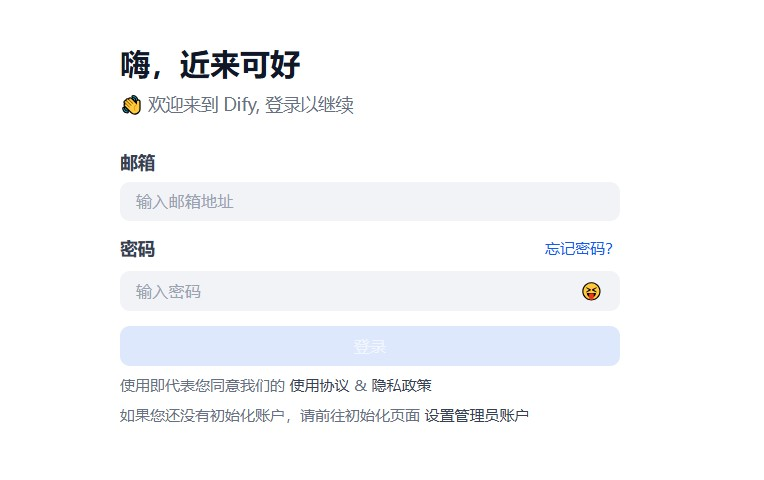
\includegraphics[width=.95\linewidth]{res/dify-login.jpg}\\
        \caption{Dify login }\label{dify-login}
    \end{center}
\end{figure}

Select models, make workflow and programming callback function of workflow

\begin{figure}[H]
    \begin{center}
        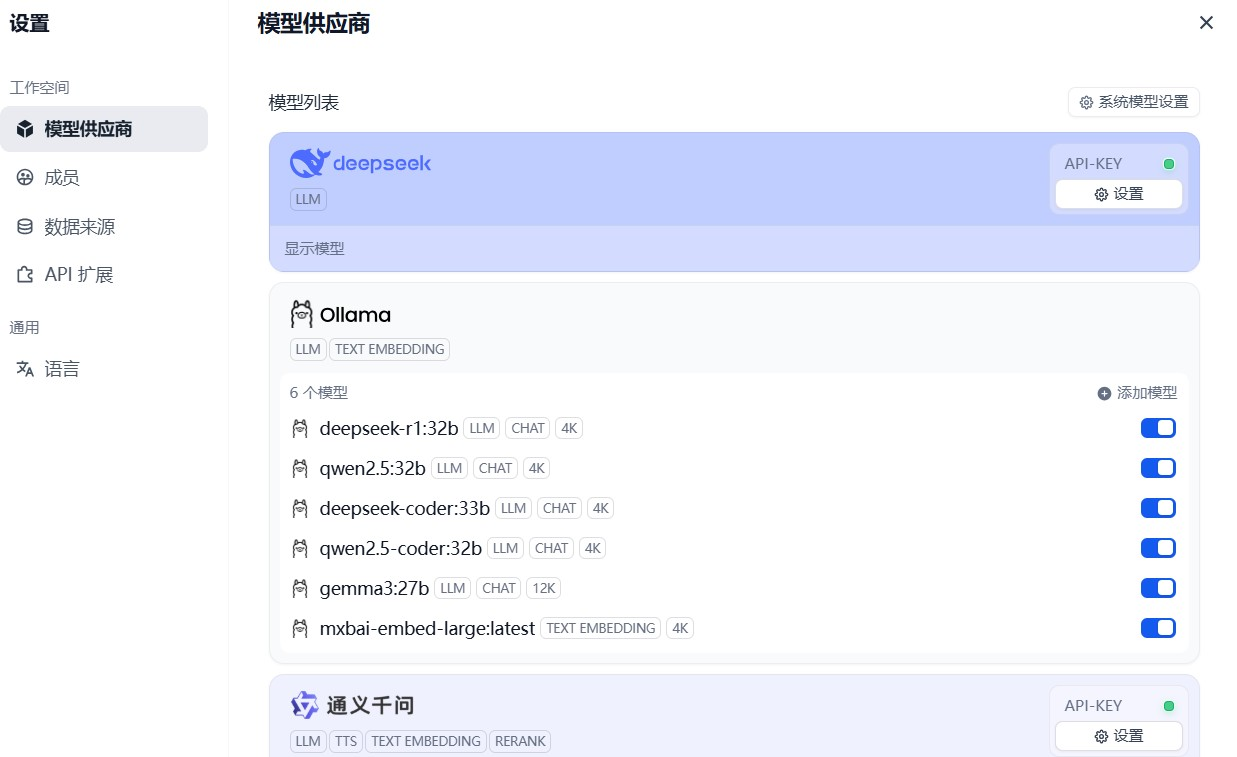
\includegraphics[width=.95\linewidth]{res/dify-models.jpg}\\
        \caption{Configure  models locally }\label{dify-models}
    \end{center}
\end{figure}

%\shortdashline

\begin{figure}[H]
    \begin{center}
        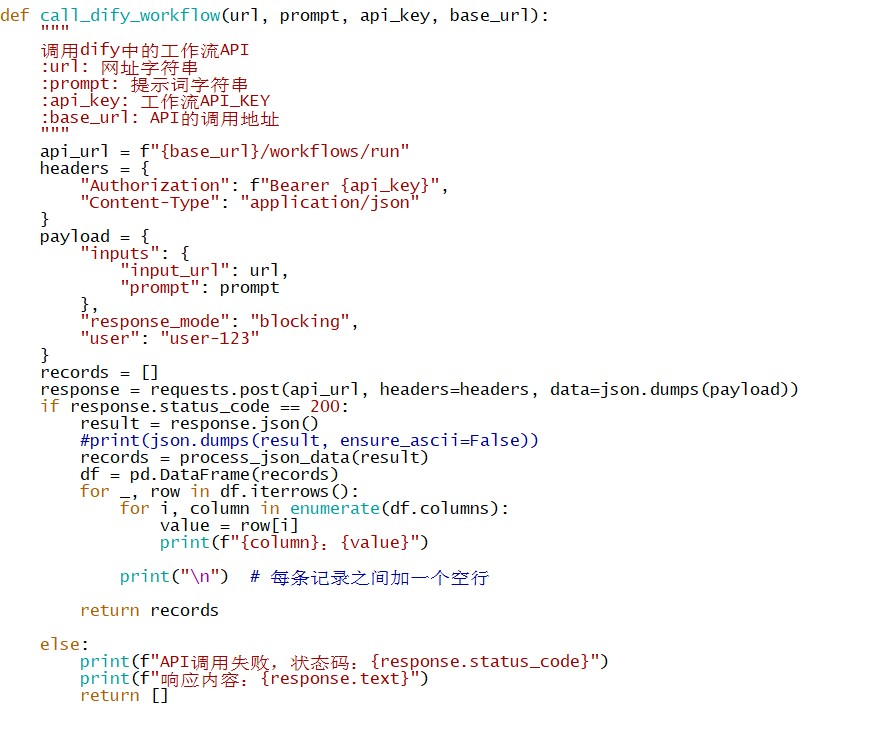
\includegraphics[width=.95\linewidth]{res/dify-callworkflow.jpg}\\
        \caption{Call back function of workflow }\label{dify-callworkflow}
    \end{center}
\end{figure}


\textbf{example 1} : example of Auto acquisition of tenders from website agent

\begin{figure}[H]
    \begin{center}
        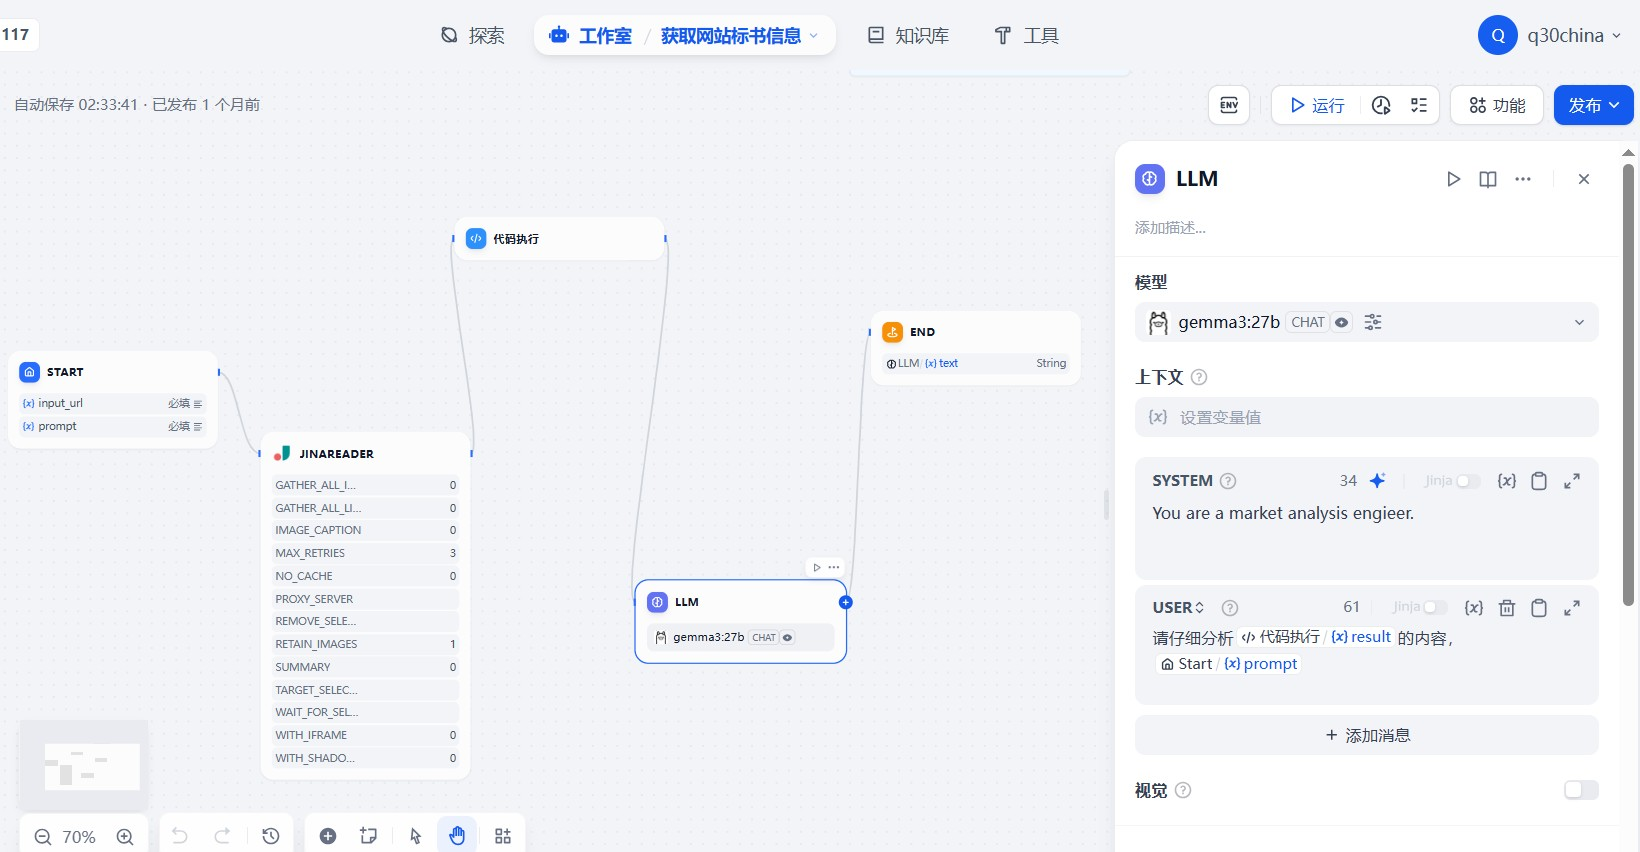
\includegraphics[width=.95\linewidth]{res/dify-tender.jpg}\\
        \caption{Workflow definition for tender acquisition }\label{dify-tender}
    \end{center}
\end{figure}

\textbf{example 2 }: example of An Testing Interview agent

\begin{figure}[H]
    \begin{center}
        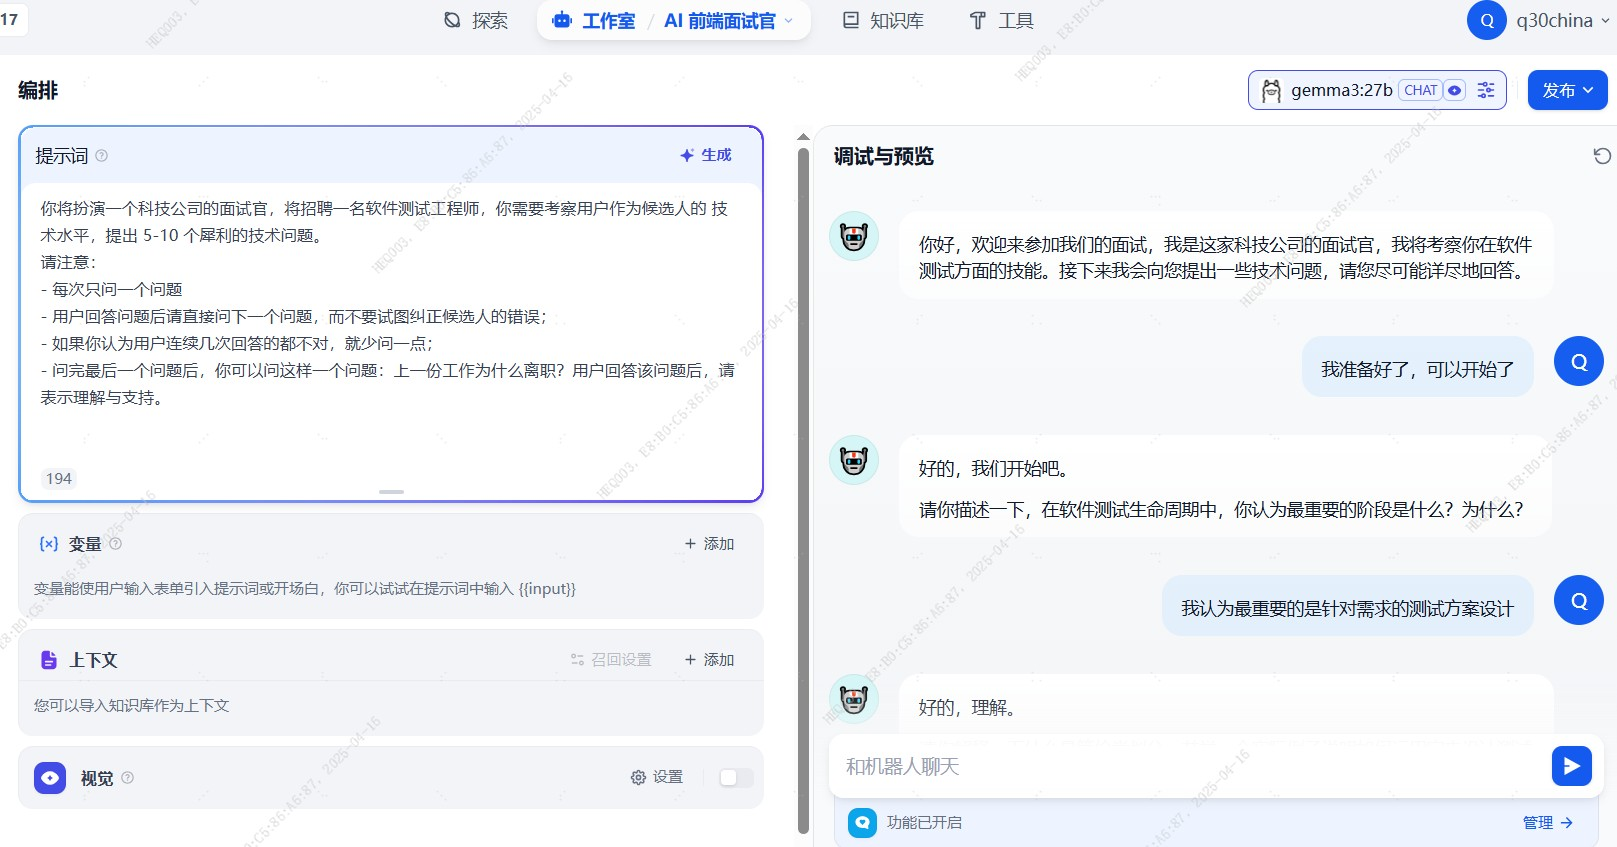
\includegraphics[width=.95\linewidth]{res/dify-interview.jpg}\\
        \caption{Interview agent demo }\label{dify-interview}
    \end{center}
\end{figure}



